% !TeX spellcheck = en_GB
% !TeX encoding = UTF-8
% !TeX program = xelatex
%----------------------------------------------------------------------------
\chapter{Methods and Implementation}
%----------------------------------------------------------------------------

\section{Graph Neural Networks on a Group FC matrix}

	\subsection{Dataset}
	\label{sec:ABIDE}
	
	The ABIDE (Autism Brain Imaging Data Exchange) dataset\cite{di2014autism} focuses on the furthering research into ASD (Autism Spectrum Disorder) through neuro-imaging and neuroscience. The dataset contains in total 1112 resting state fMRIs of subjects both with ASD (539 individuals) and typically developing controls (573 individuals). 
	
	The imaging data has been collected by 16 institutions, who collaborated to create a publicly accessible anonymised dataset to allow the broader scientific community to take part in ASD related research while preserving the privacy of the participants. As such, datasets do not contain any protected health information. 
	
	Since fMRI preprocessing techniques are very complex image processing operations and heavily resource intensive, an initiative also formed to provide a preprocessed version of the dataset. At this point I was not comfortable with taking on the connectome extraction process and so following \cite{wang2021graph}, their already preprocessed FC matrix was utilized. 
	
	These connectome matrices were extracted by first using the Craddock200 atlas and using their average correlation. After this a $k$-NN graph was constructed, keeping only the top $k$ edges for any given node, resulting in a sparser graph and creating a hyperparameter that can tune graph density.
	
	%TODO ez így nem igazán jó
	
	The very close ratio of affected vs control subjects (539 to 573) means the dataset is well-balanced in terms of a classification task on the diagnosis of subjects. 
	
	\subsection{Methodology}
	In the paper \cite{wang2021graph} by Wang et al. researchers worked with the ABIDE dataset to create a graph convolutional network based architecture for predicting the diagnosis of a patient based on the resting state fMRI. Their model 
	
	
	
	\subsection{Results}
	
	\begin{figure}[!h]
		\centering
		\begin{subfigure}[b]{0.45\textwidth}
			\centering
			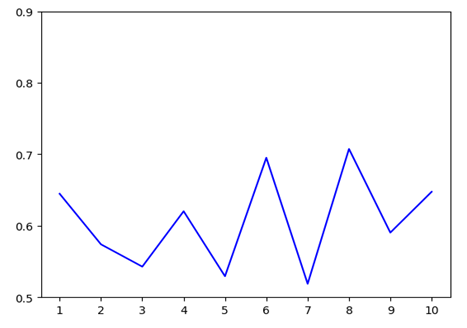
\includegraphics[width=\textwidth]{figures/onlab_results.png}
		\end{subfigure}
		\hfill
		\begin{subfigure}[b]{0.45\textwidth}
			\centering
			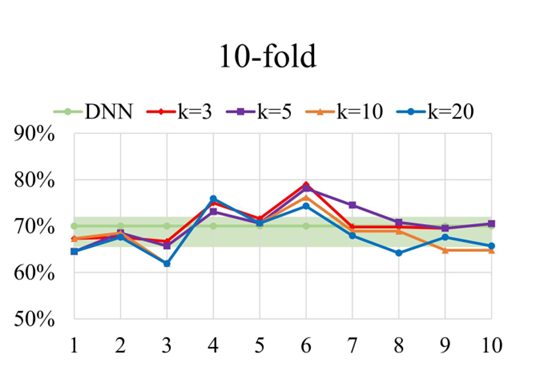
\includegraphics[width=\textwidth]{figures/paper_results.png}
		\end{subfigure}
		\caption{Tenfold crossvalidation results from my model (left) and the cGCN model from \cite{wang2021graph} (right)}
		\label{fig:onlab_results}
	\end{figure}

\section{Connectome-based diffusion}
\label{sec:diffusion}
	
	Deep learning methods are generally known for needing a large number of samples to produce the outstanding results they are capable of\cite{alzubaidi2023survey}. When working with naturally occurring data such as text and RGB images this is not quite as large of an issue, however medical
	imaging data, such MRI and CT scans, poses a problem, as it is much harder to access.
	
	In case of fMRI scans this is partly due to the cost associated with the machines and taking scans and the cost of creating high-quality datasets, as they usually require many hours of work by experts in their respective fields. Furthermore, accessing these datasets is difficult due to privacy concerns and the sensitive nature of said data\ref{sec:legal}.

	Data augmentation techniques can be used to counteract these hurdles, an important one of these is data synthesis, creating entirely new samples based previously collected data. The goal of this project was to generate synthetic three dimensional fMRI brain scans. By employing diffusion generative models it is possible to produce high-fidelity images based on previous scans.
	
	Generative models are capable of generating novel samples that they have not seen previously, based on the distribution learned from the training samples. The two types of generative models used in this model are Variational Autoencoders (VAEs) and diffusion models.
	
	Variational Autoencoders combine deep neural networks with probabilistic modelling for image generation\cite{kingma2013auto}. Instead of learning deterministic encoding, like standard autoencoders\cite{bank2023autoencoders}, VAEs learn a probabilistic representation, where the latent space follows a distribution which allows for controlled sampling and generation.
	
	A VAE is made up of two parts, an encoder and a decoder. The encoder usually consists of a series of convolutional and pooling layers to downsample the data to create a bottleneck. From this latent space, the decoder works with convolutional and unpooling (upsampling) layers to try and reconstruct the input. 
	
	Once trained, the model is capable of generating new samples by sampling from the prior distribution of the latent variable $p(z) = \mathcal{N}(0,I)$ and passing in the sample at the bottleneck to the decoder part of the model.
	
	Denoising Diffusion Probabilistic Models take inspiration from thermodynamics (particularly Langevin dynamics\cite{welling2011bayesian}) and instead of generating a sample in one step, they use a process of iterative noising and denoising\cite{ho2020denoising}. These models have become state of the art for various image synthesis tasks, producing high-fidelity results. This does come at a cost though: these models are very computationally expensive, even with further improvements, such as DDIMs (Denoising Diffusion Implicit Models\cite{song2020denoising}).
	
	During the forward noising process noise is sampled from a Gaussian distribution and added to the input image according to a noise scheduler. This process is repeated usually hundreds of times as the image shifts to a pure noise version (see Figure \ref{fig:scheduler} for examples) as the time $t$ runs from 0 to $T$.
	
	\begin{figure}[!h]
		\label{fig:scheduler}
		\centering
		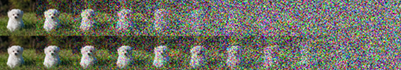
\includegraphics[width=\textwidth]{figures/scheduler.png}
		\caption{Linear (top) and cosine (bottom) noise schedulers being applied to an image of a small white dog \cite{nichol2021improved}}
	\end{figure}
	
	
	The backwards process is the task of iteratively removing noise from the destroyed image, starting from random noise. This does not have an exact solution due to information loss, so it is approximated by a neural network. The network receives the current timestep in the noising process $t$ and the image, aiming to calculate the noise, so it can be subtracted.
	
	\begin{figure}[!h]
		\centering
		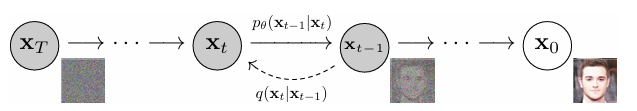
\includegraphics[width=\textwidth]{figures/diffusion.png}
		\caption{The forward and backward process of diffusion\cite{ho2020denoising}}
	\end{figure}
	
	
	Since generating in the original fMRI domain is incredibly resource intensive as the data is always at least 3 dimensional, only very small resolution samples could be generated within reasonable computation demands. The idea was to take the generative part of the model to a different space, by using a more compact representation of the brain scan: the average activation values of brain regions (ROIs) and the generated connectomes seemed like a good fit for this purpose.

	\subsection{Dataset}
	\label{sec:HCP}
	
	The HCP dataset (Human Connectome Project) was collected by WU-Minn HCP consortium. The goal of the human connectome project is to facilitate research into mapping	out the human brain, for this reason the project collected high-quality neuroimaging data (MRI, PET and MEG scans) in various studies targeting a variety of problems: Alzheimer's disease, normal brain development or ageing. In doing so they have not only supplied high quality data for neurological researchers, but also established a protocol for such data collection\cite{van2012human}.
	
	One of the collected datasets is HCP Young Adult which has scans of over 1100 healthy young adults for the free use of researchers. The dataset encompasses both resting state and task-based MRIs and was collected by 10 institutions in different parts of the world. 
	
	This work focuses on the task-based portion of the dataset, where subjects were instructed to imagine moving various parts of their body while the fMRI took place, creating 5 classes in the data based on the body part - tongue, left and right hand, left and right foot respectively. The data can be downloaded from their ConnectomeDB\footnote{\url{https://db.humanconnectome.org/app/template/Login.vm}} in an already image-wise preprocessed state as well. 
	
	Creating an easy to use dataset, where the end user wouldn’t need to have all the necessary medical knowledge and computation power to do the initial, required preprocessing steps was also a focus of the project. For this purpose common automated preprocessing pipelines were created to accomplish low-level tasks, such as surface generation, artefact removal and alignment to standard space\cite{glasser2013minimal}.
	
	\subsection{Methodology}
	
	The ROI+connectome representation first has to be extracted from each sample of the dataset and then they are used as the input for the diffusion model. Since the connectome at this point is not an image but rather a sort of brain graph, a decision has been made to create a model different from most DDPMs, by creating a specialized graph U-net, that can serve as the neural network inside the diffusion model that predicts the noise. To do this, I adapted the original graph U-net\cite{graph-u-net} to work in this setting, by adding time and class conditioning and edge prediction techniques.
	
	The resulting generated connectomes and ROI values are then used as conditioning in the bottleneck of a VAE, which has been trained to generate MRI scans with the original images of the same dataset, using the original ROI and connectome values as conditioning during training. 
	
	Here, the goal was to make sure the VAE learns how to generate scans that correspond to the information fed at the bottleneck; this way it is possible to generate ROI and connectome samples, which can be turned into high-fidelity MRI samples with significantly less resource usage than if we were generating the MRIs in the first place.
	
	\subsubsection{Data Preprocessing}
	
	The architecture requires three separate types of data: the fMRI scan itself and the ROI values and connectomes corresponding to the scan. Of these the HCP dataset only contains the preprocessed fMRI scan, the other two needed to be computed in a preprocessing pipeline\ref{sec:extract}. The ROI values were extracted with the help of an atlas, which describes the regions of the brain corresponding to the ROI values. Since the focus of the project was on sensory motor tasks, therefore we filtered for brain regions activated during these tasks (in practice this means 21 ROIs for each side of the brain, so 42 altogether). 
	
	With the filtered atlas, a mask can be constructed, to block out unwanted parts of the brain during the extraction. Understanding the format and meaning of the data used in the preprocessing (e.g.: What ROIs and connectomes are and how to calculate them) is difficult as it requires knowledge in the medical domain. 
	
	The correct preprocessing was possible thanks to communication from doctors, the documentation of the nilearn package and high-quality HCP dataset. Due to the preprocessing of the dataset, it works best with the Glasser360 brain atlas\cite{sporns2005human}, which was constructed using HCP data and identifies 180+180 (in the left and right hemisphere) regions of interest according to changes in cortical architecture, function, connectivity, and/or topography.

	\begin{figure}[!h]
		\centering
		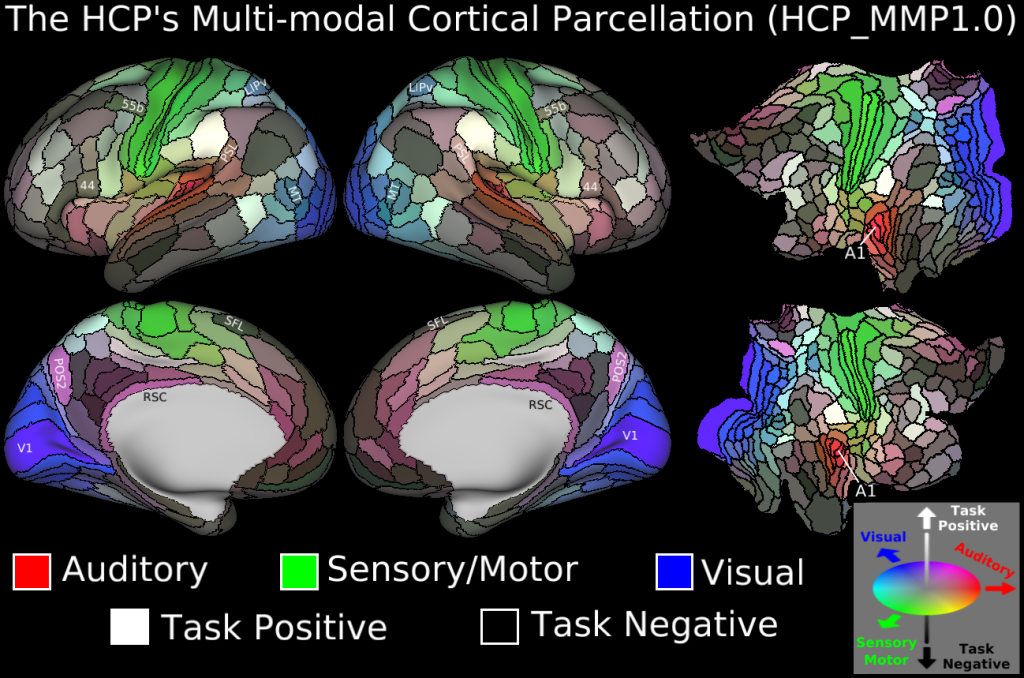
\includegraphics[width=0.8\textwidth]{figures/atlas.png}
		\caption{The Glasser360 brain atlas created based on the HCP healthy adults dataset\cite{sporns2005human}}
	\end{figure}

	After the extraction is complete we get a timeseries of ROI values for each patient. This means a tensor of size $284 \times 16 \times 42$, (time $\times$ repeatedMeasurements $\times$ ROIs). To validate the correctness of the preprocessing a Support Vector Machine was used to classify the ROIs based on the performed task. For this the ROI values need to be standardized per subject, and separated by task. For this a Python script from previous works was used that generates a csv file with the times slices and the task performed at that time interval. 
	
	This file is essential in separating the relevant parts of the scans from the noise where no task is performed. The scans contain measurements for 5 tasks performed twice, so in to 10 for
	each patient, with 16 repeated measurements take by the MRI machine (As a further preprocessing step, before the data was used in models the mean value of these 16 steps was taken). This means 124 of the 284 long
	scan is noise.
	
	Once the preprocessing was correct the SVM achieved 90-95\% accuracy on the classification task based on performed tasks. For calculating the connectomes from the ROI values the nilearn package’s ConnectivityMeasure class was used. 
	
	The subject-wise calculated ROIs were separated by tasks and connectomes were calculated for each task separately. Since measurements across different tasks are differ significantly, calculating the connectomes with the tasks mixed would not yield meaningful results.
	
	\subsubsection{Proposed Architecture}
	
	The model consists of a diffusion block and an autoencoder. The diffusion block is trained on the ROI values and connectomes to also generate ROI values and connectomes, which are used to condition the autoencoder at the bottleneck.
	
	\begin{figure}[!h]
		\centering
		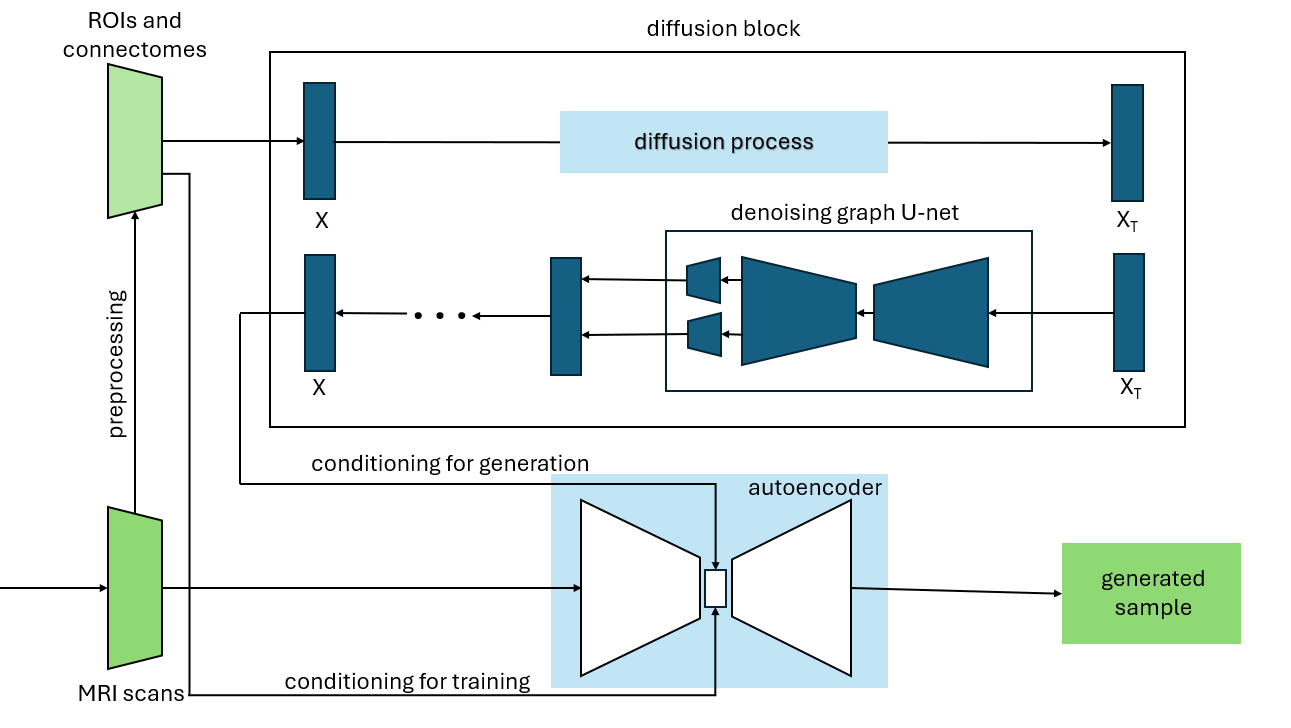
\includegraphics[width=\textwidth]{figures/architecture.png}
		\caption{Visualization of the model architecture, focusing on the flow of data}
	\end{figure}
	
	A big advantage of this model is that the two parts of the model can be trained separately. The autoencoder is trained to be able to reproduce scans with the corresponding connectome. At sampling time  the two models are used in conjunction: the diffusion model generates a connectome and only the decoder part of the autoencoder is used to generate novel samples.
	
	For the DDPM and DDIM diffusion blocks the implementation in the denoising-diffusion-pytorch package was used to enable quick experimentation. The package provides an easy interface to train diffusion models with custom networks, though it required some unused parameters to be added to model, that were unnecessary in this use-case.
	
	Another advantage of this package is that it enables easy DDIM sampling. This could be used with 200 steps, instead of the 1000 used for training the DDPM. This package sadly lacks the capability for training a network with class conditioning, so for experiments involving class conditioning it was extended manually.
	
	For a VAE implementation, since it is not a focus of this work, a choice was made to use an implementation provided by the latent-diffusion Github repository\footnote{\url{https://github.com/CompVis/latent-diffusion}}. The model this library provides has the option to train a VAE that learns representations on 3D data. 
	
	The class was modified in minor ways to fit in with the rest of the codebase and  two major changes had to be made to it. Firstly,  the loss function was recalibrated to enable the model to train on the given dataset. Secondly, it was extended with the capability to condition the bottleneck with the ROI values and connectomes. 
	
	For the conditioning a small CNN was implemented with a fully connected layer at the end, that takes the 2 × 42 × 42 size ROI and connectome tensor and creates an embedding with the same size as the bottleneck. The conditioning is then implemented by performing Adaptive Instance Normalization\cite{huang2017arbitrary} on the embedding and the values in the bottleneck.
	
	\subsubsection{Graph U-net}
	
	U-nets are a very successful subtype of CNN architectures, originally invented with the purpose of biomedical image segmentation\cite{ronneberger2015u}. It is widely used in segmentation tasks and other cases where the output needs to have the same dimensions as the input, due to its symmetrical nature. This is the same reason why they're commonly used in diffusion models as the noise prediction neural network\cite{ho2020denoising}.
	
	\begin{figure}[!h]
		\centering
		\label{fig:unet}		
		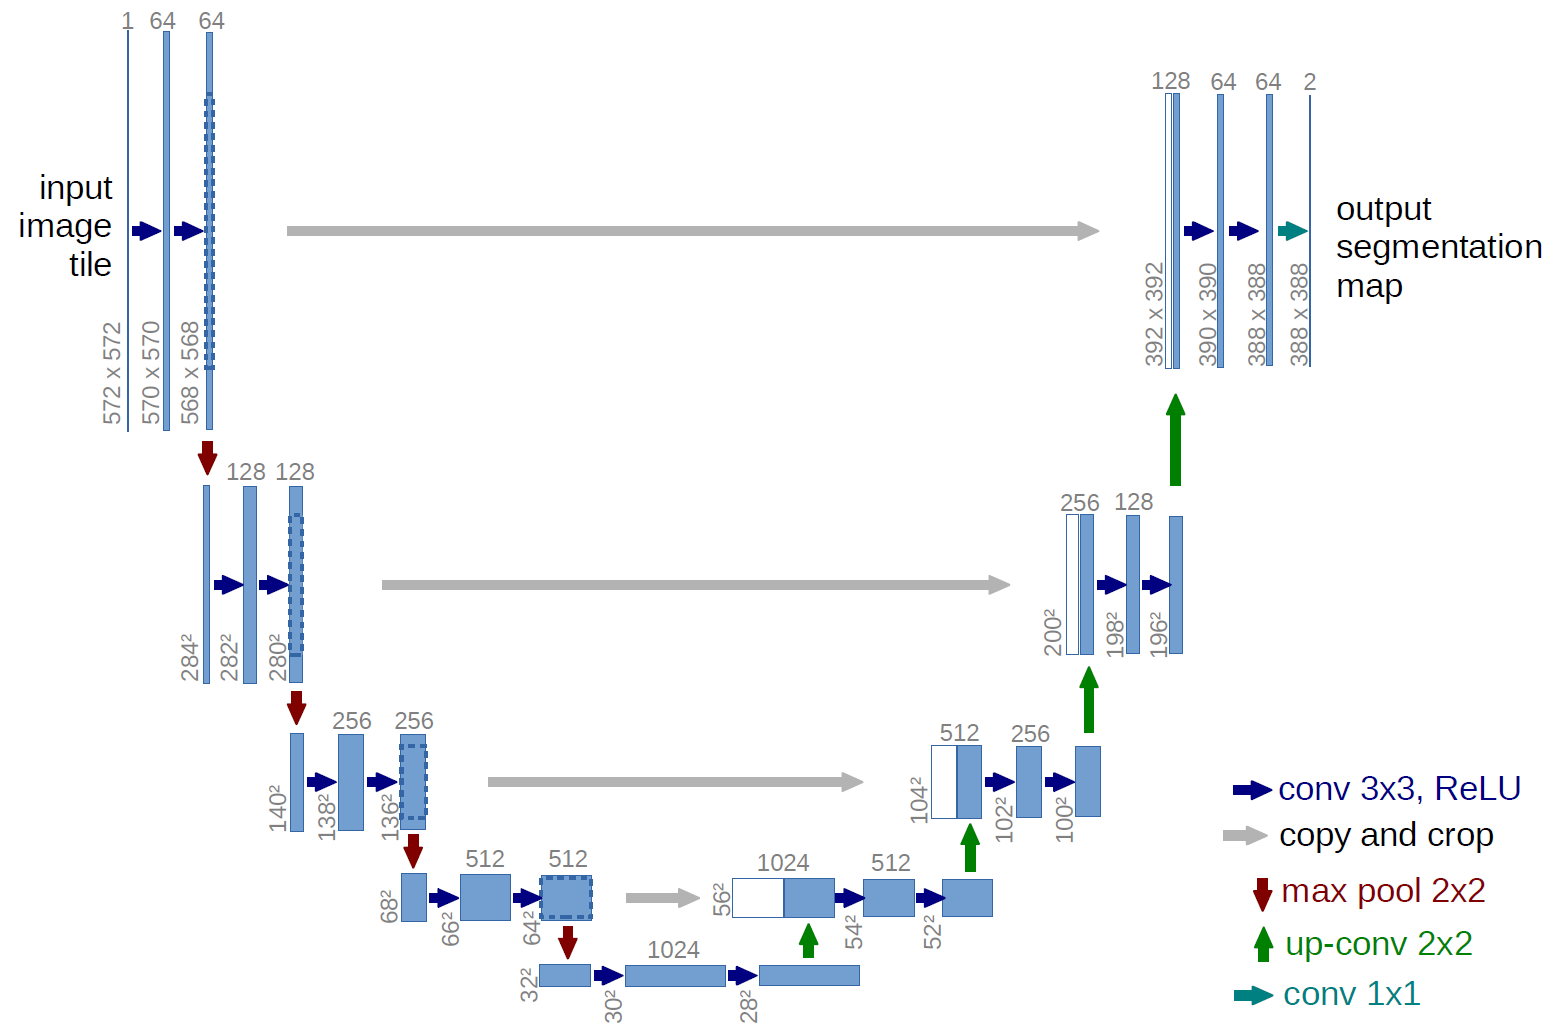
\includegraphics[width=\textwidth]{figures/u-net-architecture.png}
		\caption{Visualisation of the U-net architecture\cite{ronneberger2015u}}
	\end{figure}
	
	
	U-nets are named due to their distinctive architecture: the network consists of a contracting and expansive path, which together form a u-shape (Figure \ref{fig:unet}). The contracting path is a typical CNN with convolutions and max pooling. Conversely the expansive path has upsampling and convolutions, while skip connections are also utilized where dimensions match.
	
	Since U-nets have been such a successful model type in convolutional networks, there has been an effort to find an analogue in graph convolutional networks as well. Graph U-nets\cite{graph-u-net} follow the original principles of the U-net architecture: the encoder-decoder structure, the skip connections and the general architecture, as seen on Figure \ref{fig:gunet}. 
	
	The convolutional layers are replaced by GCN layers and for standard pooling and unpooling layers which do not have an obvious graph equivalent, since they rely on locality in images that is not present in general graphs, novel layers have been developed for graph pooling and unpooling.
	
	\begin{figure}[!h]
		\label{fig:gunet}
		\centering
		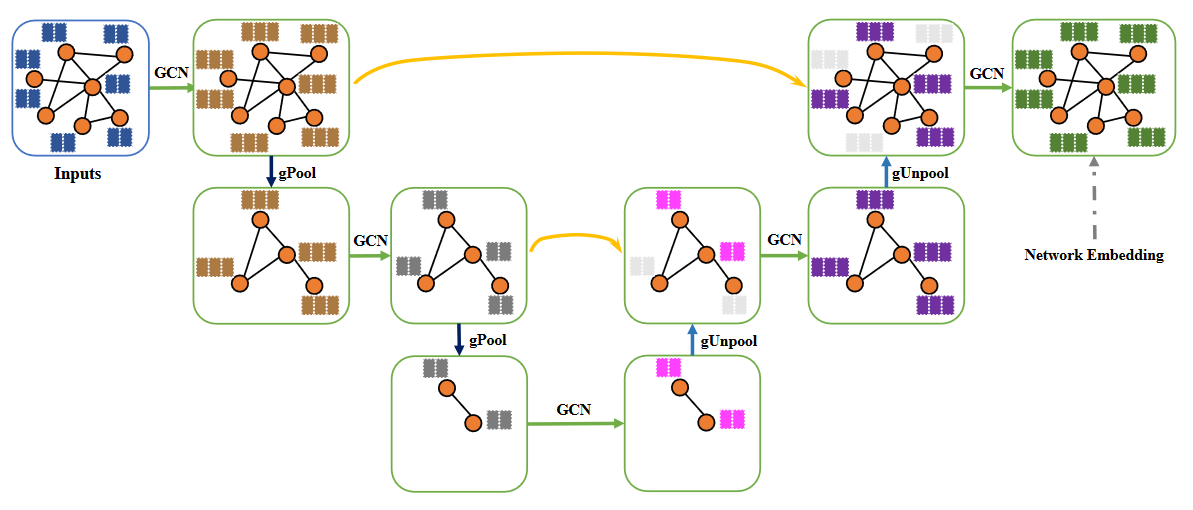
\includegraphics[width=\textwidth]{figures/gunet.png}
		\caption{Visualization of the graph U-nets architecture\cite{graph-u-net}}
	\end{figure}
	
	Graph pooling layers enable downsampling on graphs by adaptively selecting nodes to build a smaller graph from existing nodes, while preserving edges. The selection method is similar to a traditional $k$-max pooling: the highest $k$ values are preserved after the operation. The top $k$ nodes are selected based on a learned 1D projection, to a vector $\textbf{p}$:
	
	
	$$ y_i = x_i\textbf{p}/||\textbf{p}||, $$
	
	the nodes are kept which retain most of their information when projected to \textbf{p}. After the selection has been made, the adjacency matrix is updated to only include these nodes and the corresponding rows are extracted from the feature matrix via a gate operation, using matrix multiplication and a sigmoid operation, which makes p trainable by backpropagation.
	
	
	The unpooling layer, unlike image upsampling layers, can only work in connection with a graph pooling layer for which it performs an opposite action: the adjacency matrix is restored to its state prior to the the pooling layer and the node feature matrix is distributed into a shape corresponding to this larger number of nodes, having zero values for newly reappearing nodes.
	
	The graph U-net used in our model is a modified version of the architecture proposed in \cite{graph-u-net}. The connectome is used as the adjacency matrix in the U-net, the connectivity values between ROIs are the weights of edges in the graph. 
	
	Since we have singular ROI values available for each of the nodes these were distributed along an identity matrix to create a better node feature input for the network, and since the U-net requires symmetry and we will be looking to generate both connectomes and ROI values, the full input is the concatenation of the ROI filled identity matrix and the connectome. 
	
	In this case, since the connectomes are $42 \times 42$, the input of this part of the network is batch size $\times 42 \times 84$.
	
	
	The model has the same number of blocks in both directions, comprised of one GCN layer and one graph pooling layer in the down direction and one graph unpooling layer and one GCN layer in the up direction, with a connecting bottom GCN layer. 
	
	Corresponding blocks of the same size are connected via skip connections. Conditioning (with the main concern being time conditioning) is applied at every block by calculating scale and shift vectors via a small MLP.
	
	
	The output of the last block is thus the same size as the input of the first one and it gets separated into node features that are used for ROI values calculation and node features that are used for connectome calculation. The ones used for ROIs are sent through a final GCN layer where they are reduced to single value per node and then distributed along an identity matrix to preserve the symmetry of the data. 
	
	For the connectome however, as each value represents an edge between two regions, the other half of the output gets pairwise concatenated and passed through an MLP to determine one value per edge for the connectome.
	
	\begin{figure}[!h]
		\centering
		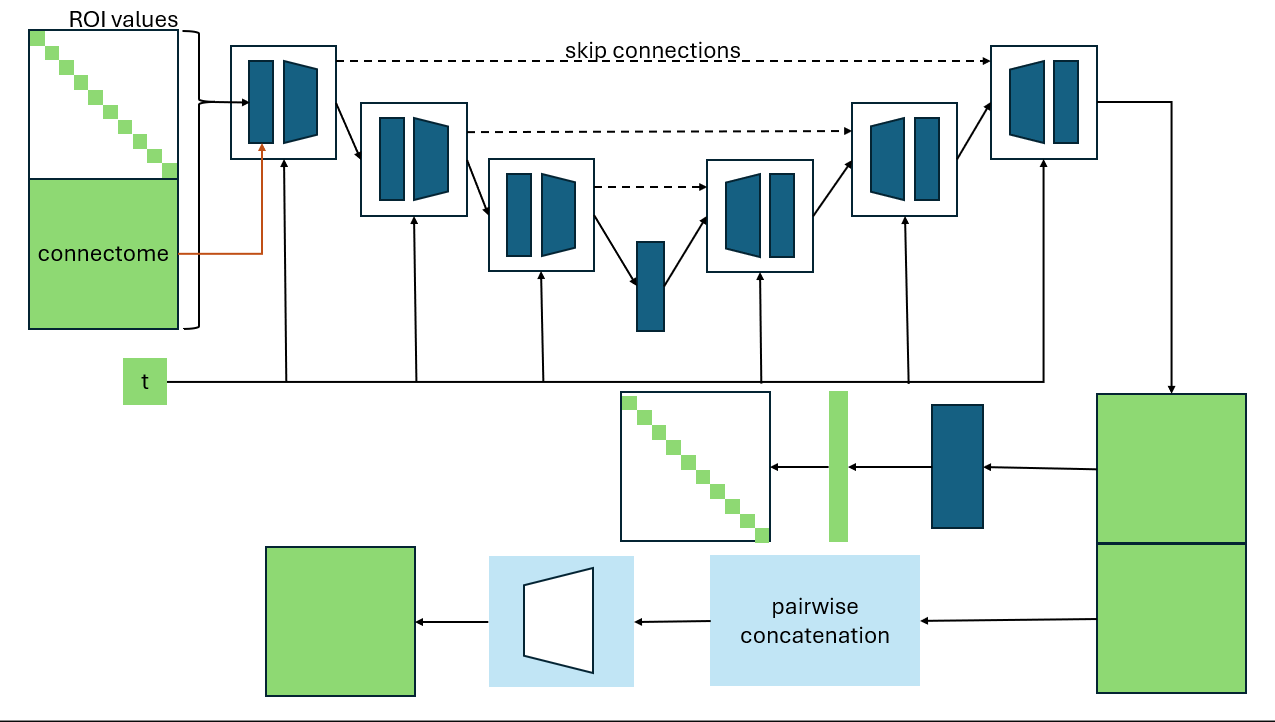
\includegraphics[width=\textwidth]{figures/own_gunet.png}
		\caption{Visualization of the graph U-net architecture, focusing on the flow of data}
	\end{figure}
	
	
	\subsubsection{Experiments}
	
	To find out which choices work best for the model, there were multiple experiments with various architecture and parameter ideas. This was mainly focused on the graph U-net, as it is the central part of the architecture. The VAE remained largely the same, with only minor changes to accommodate the conditioned training and sampling.

	\textbf{Graph U-net} Since this kind of graph U-net and diffusion architecture does not show up in literature often, experiments were done to try and figure out which setups would lead to better generation results in the end. There were wide variety of options to try and the lack of guidance on which ones could be successful in which combination meant trying out new ideas in a fail fast method would be best: the results of the model were inspected after a set number of epochs and if the connectome visually worsened that method could be avoided in the future.
	
	The usual output of a graph u-net is just node features and there are various methods to convert them into edge predictions\cite{li2023evaluating}, therefore it was important try a few to see what would work well with the model. In the implementation of the graph U-net I have included a switch that can take None, ’scalar’ and ’mlp’ values and makes experimenting with this easier. 
	
	The None value keeps the original vector of the output, without any transformations applied. In this setting the network tries to learn the noise as if they were features of the nodes, both for ROI values and edge weights. This is the easiest method to implement but this way it is not taken into consideration how each edge represents the connection between two nodes.
	
	To better represent the way a connection is formed between two nodes, the ’scalar’ method takes each resulting node embedding and computes the scalar product of each node pair to build the new adjacency/edge weight matrix. In case of the ’mlp’ option the node embeddings get pairwise concatenated to represent their respective edges, and then are passed through a small MLP to calculate an edge strength for the pair of nodes. Here the concatenation makes sure that both nodes are considered together in the calculation.
	
	
	The most usable and best performant solution for calculating the connectome ended up being the MLP, as it yielded better results than the base method and the scalar product approach seemed to lead to generated samples looking almost identical.
	
		
	\begin{figure}[!h]
		\centering
		\begin{subfigure}[b]{0.45\textwidth}
			\centering
			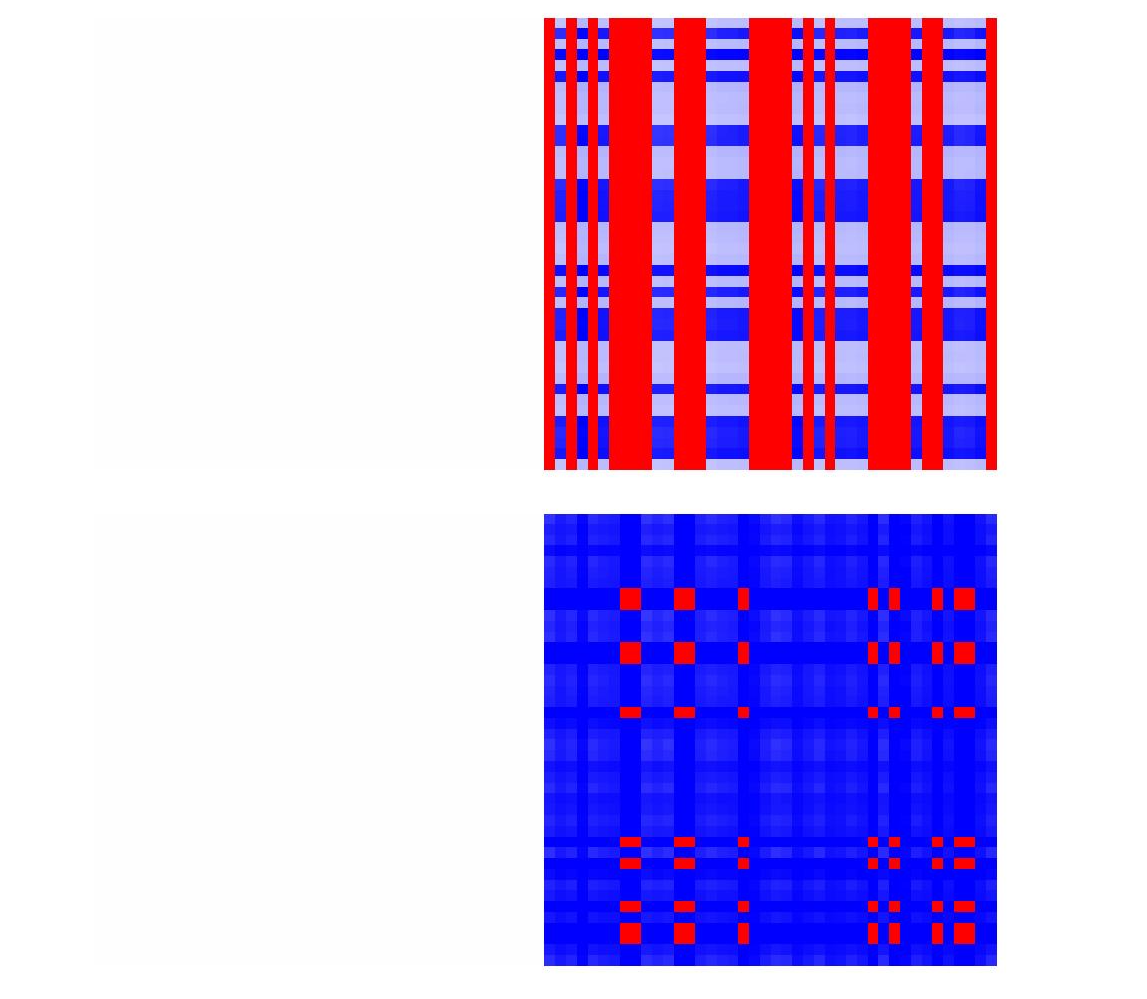
\includegraphics[width=\textwidth]{figures/bad.png}
		\end{subfigure}
		\hfill
		\begin{subfigure}[b]{0.45\textwidth}
			\centering
			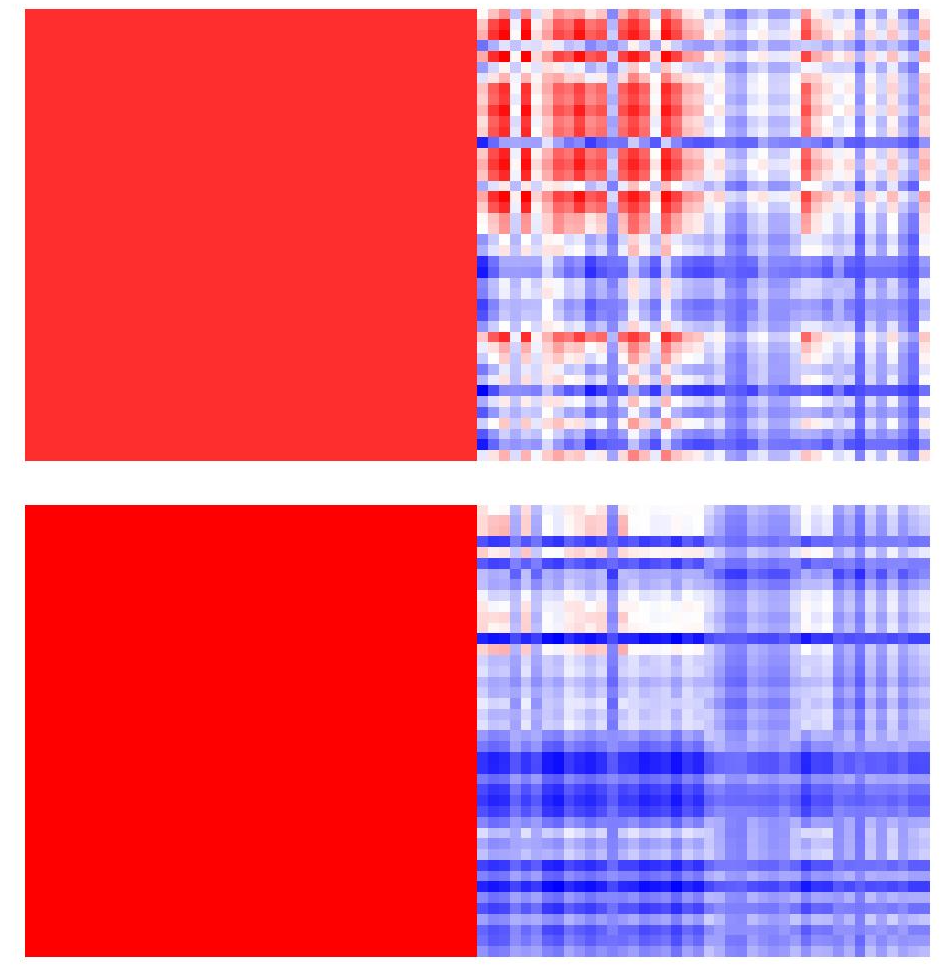
\includegraphics[width=\textwidth]{figures/bad2.png}
		\end{subfigure}
		\caption{Bad generated ROI activation values (left) and connectomes (right).}
		\label{fig:bad-samples}
	\end{figure}
	
	
	
	\textbf{Class conditioning} Conditional diffusion models enable generating images with specific features. In case of class conditioning the model is tasked with generating a sample from a category from a list that is already known ahead of time. This can be achieved by passing an embedding of the class labels to the noise predicting network. This approach guides the model to learn the different characteristics of each class, which usually leads to better overall image quality. It also grants the ability to generate images for specific classes, which is especially useful in the medical domain.
	
	Since the used dataset has labels in form of the body part corresponding to the performed task, it was possible to add this technique into the model. A very simple implementation of this was constructed, by passing the class label to the U-net, where it was turned into a one-hot vector and concatenated to the time conditioning to perform both at once.
	
	Unfortunately this implementation did not result in improved performance, the resulting generated samples tended to have prominent bands of a single value instead of resembling the original samples. It could still be a good idea to further experiment with class conditioning, perhaps with a different implementation method. 
	
	Since the connectome is supposed to be a symmetric matrix, the graph U-net’s loss function could be changed in some way to reflect this in some form. A version of loss calculation was tried out, where only the lower triangle matrix of both the result and target were considered during calculation: keeping the generation of the upper half as a sanity check, but concentrating on the lower half. This did not noticeably impact the resulting generated samples, so it was removed, choosing to keep the model simpler if possible.
	
	\subsection{Results}
	
	To evaluate image generation tasks, it is best to use multiple different approaches. On one hand, quantitative metrics like Fréchet Inception Distance\cite{heusel2017gans} (FID), Peak Signal to Noise Ratio\cite{hore2010image} (PSNR), and Structural Similarity Index Measure\cite{hore2010image} (SSIM) are important to obtaining an objective view of the quality of the generated images. On the other hand, especially in image synthesis tasks, qualitative evaluation is important to assess the visual quality of the samples, as numerical measurements don’t always align with visual representations.
	
	
	FID uses an InceptionV3\cite{szegedy2016rethinking} network to calculate the distance between the extracted features of real and generated samples, PSNR measures the ratio of the signal (i.e., the important parts of the image) and noise in the reconstructed image, and SSIM, unlike PSNR, measures not the pixel values, but structural aspects of the samples.
	
	As a baseline, we can compare these metrics to those measured on a pixel-based 3D DDPM architecture\cite{diff_pixel}:
	
	\begin{table}[!h]
		\begin{center}
			\begin{tabular}{lccc}
				\toprule
				Method & FID & PSNR & SSIM \\
				\midrule
				Ours & 400.8233 & 13.4702 & 0.0535 \\
				Pixel-based & 20.4152 & 27.5278 & 0.8442\\
				\bottomrule
			\end{tabular}
		\end{center}
		\caption{Comparison of results on quantitative metrics between our method and a pixel-based DDPM method.}
	\end{table}
	
	From these numerical metrics it is obvious that the results of the architecture are not comparable to the results achieved by using the diffusion to generate the fMRI sample directly. 
	
	\begin{figure}[!h]
		\centering
		\begin{subfigure}[b]{0.45\textwidth}
			\centering
			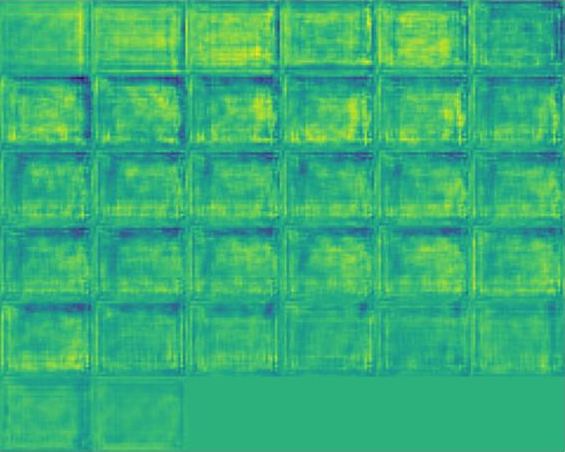
\includegraphics[width=\textwidth]{figures/bad-vae-sample.png}
		\end{subfigure}
		\hfill
		\begin{subfigure}[b]{0.45\textwidth}
			\centering
			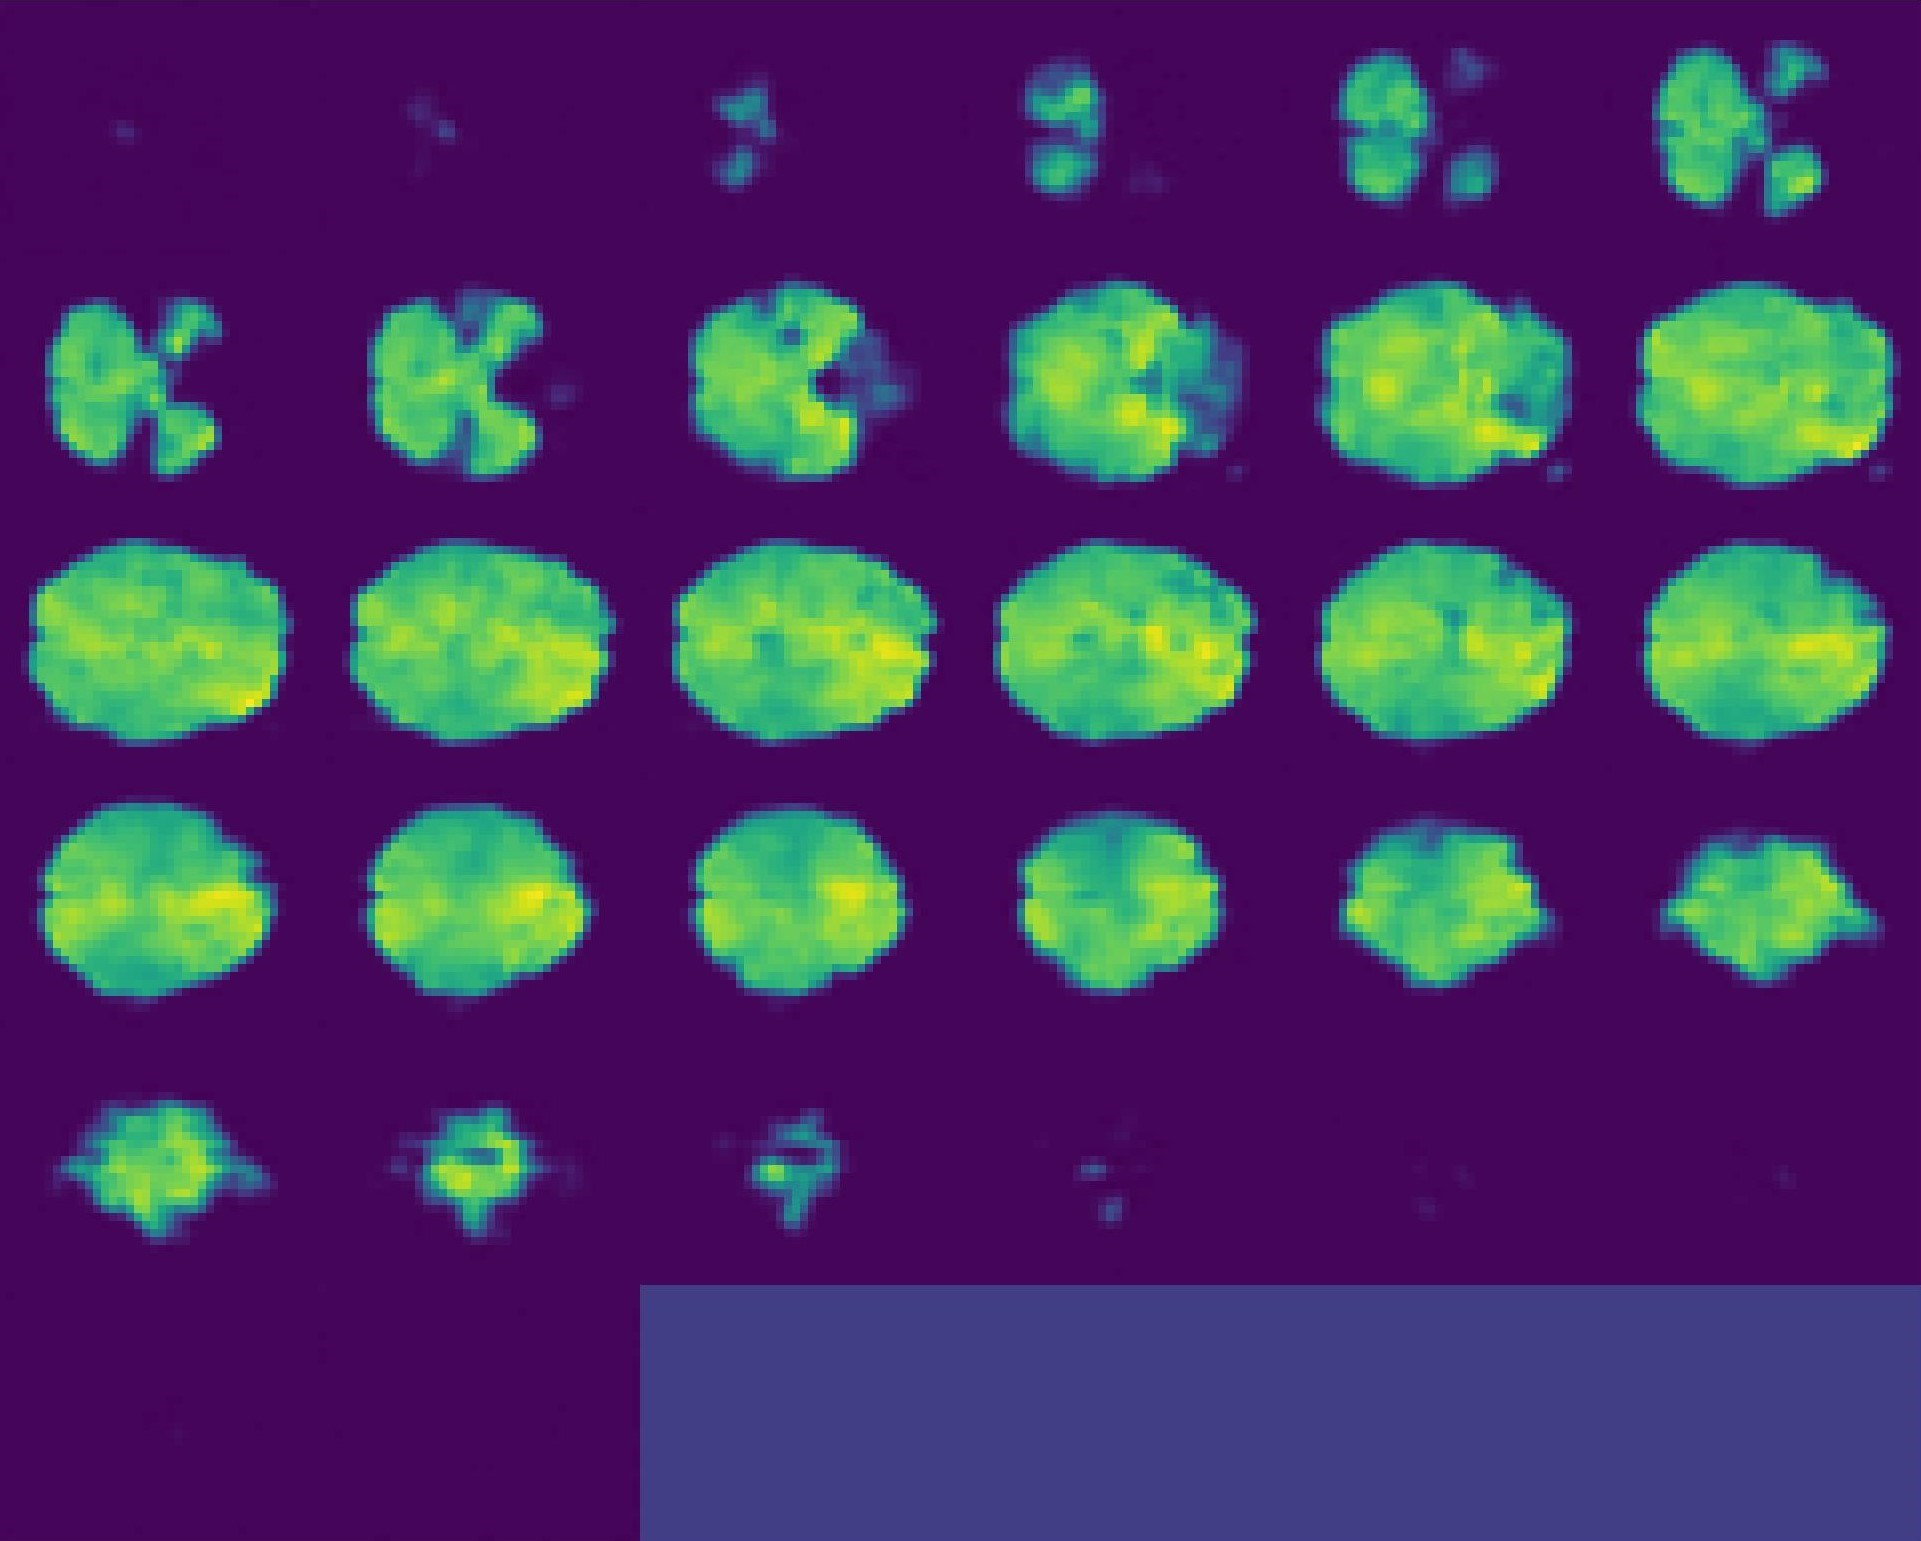
\includegraphics[width=\textwidth]{figures/good-vae-sample.jpeg}
		\end{subfigure}
		\caption{Samples from the VAE, on the left a sample generated by the decoder conditioned by generated BOLD signals, on the right a sample generated during a validation epoch.}
		\label{fig:vae-samples}
	\end{figure}
	
	
	As it can be seen on Figure \ref{fig:vae-samples}, the trained VAE was capable of generating reasonably good samples in validation epochs when conditioned with one of the original connectomes. It has some artifacting and small chunks outside of the brain, but it looks very similar to the input images. The left sample however, the one conditioned by synthetic data is very noisy and does not resemble samples from the training dataset. This comparison points to our generated ROIs having the opposite of the desired effect, as they completely destroy the image.
	
	\subsection{Conclusions}
	
	To understand the poor performance of image generation, we have to examine the results of the connectome and ROI value generation. The training of the model was very unstable, often devolving into a mass of low and high values in various patterns (as seen on Figure \ref{fig:bad-samples})
	This has become worse in later epochs, as the model could produce promising results after ~20 epochs of training, as seen on Figure \ref{fig:roi-samples}. 
	
	Overall, this seems to suggest that there is potential for good outcomes in the model architecture but there is some sort of numerical or gradient instability that causes it not to converge. This is backed up by how the loss behaves during training. It can be seen on Figure \ref{fig:loss} that while the loss initially drops many orders of magnitude at the start of training, after zooming in it is obvious that the loss still jumps around and does not actually converge.
	
	\begin{figure}[!h]
		\centering
		\begin{subfigure}[b]{0.4\textwidth}
			\centering
			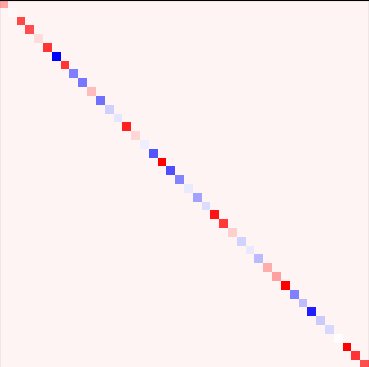
\includegraphics[width=\textwidth]{figures/training-roi.png}
		\end{subfigure}
		\hspace{-1em}
		\begin{subfigure}[b]{0.4\textwidth}
			\centering
			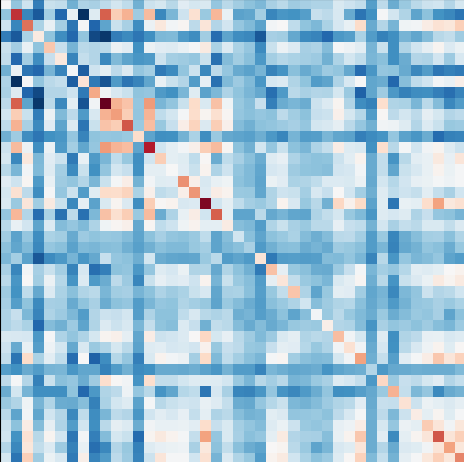
\includegraphics[width=\textwidth]{figures/training-connectome.png}
		\end{subfigure}
		\par\bigskip
		\begin{subfigure}[b]{0.8\textwidth}
			\centering
			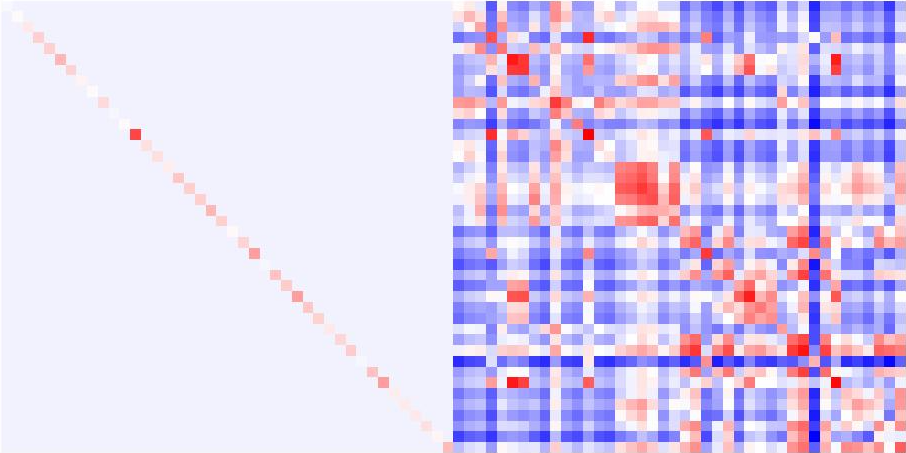
\includegraphics[width=\textwidth]{figures/good-roi-sample.png}
		\end{subfigure}
		\caption{On the bottom is one of the better samples generated by the model, and on the top a sample from the training dataset. ROIs are on the left and connectomes are on the right.}
		\label{fig:roi-samples}
	\end{figure}
	
	While the network is not capable of generating consistently good, novel samples in its current state, there is reason to believe that with the right adjustments this architecture could be capable of learning meaningful representations of the data. Other than this, this idea is a great step in resource intensiveness. It has about 80\% less parameters than a pixel-based diffusion model using 3D-Unet would. It also decouples the diffusion process from the slower, more costly pixel-based VAE, which enables rapid experimentation: once trained, a VAE can be used to test out many GNN models.
	
		\begin{figure}[!h]
		\centering
		\begin{subfigure}[b]{0.45\textwidth}
			\centering
			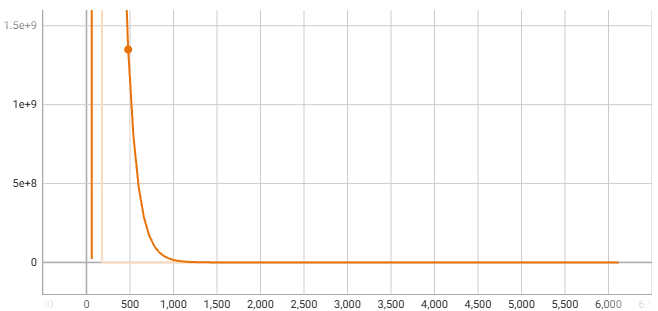
\includegraphics[width=\textwidth]{figures/train-loss.png}
		\end{subfigure}
		\hfill
		\begin{subfigure}[b]{0.45\textwidth}
			\centering
			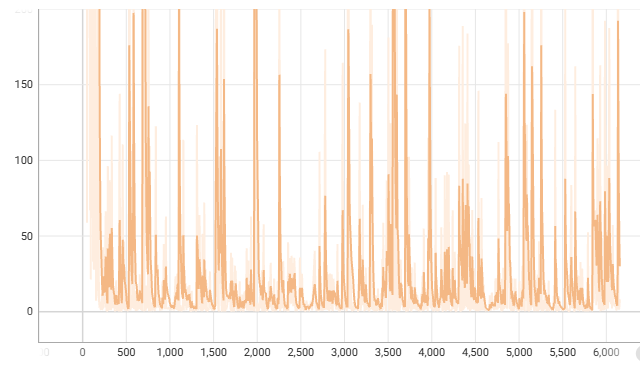
\includegraphics[width=\textwidth]{figures/step-loss.png}
		\end{subfigure}
		\caption{Loss during training.}
		\label{fig:loss}
	\end{figure}

\section{Exploring device-to-device differences}

	Most publicly available larger fMRI datasets are a result of large-scale collaborations of various healthcare and academic institutions (like the ones described in Section \ref{sec:ABIDE} and \ref{sec:HCP}), since collecting this many scans is both very resource intensive and takes a long time. These collaborations are incredibly valuable data sources, but this also results in a crucial characteristic: the fMRI scans are from different machines.
	
	These machines are very precise and well-engineered devices and the scan settings are coordinated to be the same across all study participants, but there can be variances in the different machines and environmental factors that lead to small differences in scans\cite{sutton2008investigation} that can lead to different performance in machine learning applications. If this is the case it could be helpful to introduce a preprocessing step that neutralizes this issue.

	\subsection{Dataset}
	
	My experiments were conducted on the ABIDE dataset\cite{di2014autism} (same as in Section \ref{sec:ABIDE}). More specifically to avoid costly preprocessing steps, but to be able to be keep in control of the connectomes and other facets of the resulting data, I turned to the Preprocessed Connectomes Project (PCP) initiative's ABIDE preprocessed dataset\cite{craddock2013neuro}.
	
	Since there is not a widely accepted best practice method for preprocessing fMRI images, the participating five teams have all used their preferred methods to clean the data and various derivatives of this process are downloadable from the provided Amazon S3 bucket. From my perspective, the most important of these is the ROI activation timeseries: for each preprocess method, the resulting preprocessed scans were segmented using 7 different brain atlases. 
	
	I built the used dataset from these activation timeseries using methods outlined in a paper about the NeuroGraph dataset\cite{said2023neurograph}. In this paper researchers argue that the reason applying GNNs in the neuroimaging domain has been so challenging is the expansive number of different preprocessing pipelines and the large parameter search space. To counteract this problem, they benchmarked various representations with the most commonly used GNN architectures to offer guidance for dataset construction.
	
	For their experiments they used the HCP dataset (See Section \ref{sec:HCP}) and constructed five different tasks, each with corresponding datasets with different parameters. Through their benchmarking efforts they have found that a larger number of regions of interests, creating sparser graphs and using the correlation matrix as node features leads the best results across tasks and network types. This is invaluable information for further research and it would have been very beneficial, had I known about it in previous endeavours.
	
	For the construction of this dataset, I have followed these suggestions. First the timeseries needed to be normalized to a zero mean and unit variance for each subject individually. With the help of nilearn, the correlation was used to create graph structure and the node features. For the graph structure, only edges running between nodes with a positive correlation were kept and a hyperparameter was introduced to keep only the top $n\%$ of edges with the highest correlation leading to sparser graphs. For edge features the original correlation matrix was kept.
	
	\subsection{Methodology}
	
	In the ABIDE preprocessed dataset samples are also categorized by the performing institution. To better understand the impact of the specific machine being used on the data, in this experiment I have used the most numerous sites to create a dataset that focuses not only predicting diagnoses, but also on this aspect. As it is visible on Figure \ref{fig:distribution}, there are only a few sites that have a considerable amount of samples on their own. The decision was to use the ones with over 100 samples: NYU (NYU Langone Medical Center), UM\_1 (University of Michigan: Sample 1) and USM (University of Utah School of Medicine).
	
	\begin{figure}[!h]
		\centering
		\label{fig:distribution}
		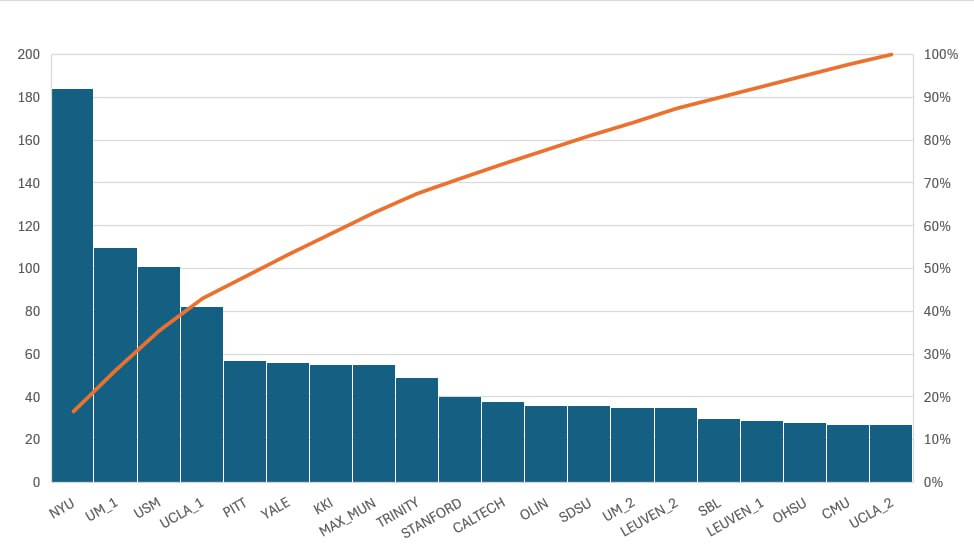
\includegraphics[width=0.8\textwidth]{figures/ABIDE-sites.jpg}
		\caption{The distribution of capturing site within the ABIDE dataset.}
	\end{figure}
	
	%TODO írni a modellről
	In creating a model for this task, the guidance from \cite{said2023neurograph} was followed similarly as to before. This study found that residual- (or skip-) connections play a pivotal role in enhancing the performance of brain networks.
	
	The tests were performed using the three institutions' samples: on one hand, with each of the three sets separately and together with the test set randomly separated from the train set, on the other hand with a leave-one-out method. In the latter, one of the sites is left out of the training set and kept exclusively for testing: this can be a good way to measure how effectively the model can learn patterns that are also applicable in data from previously unseen sites.
	
	\subsection{Results}
	
	
	
	\subsection{Conclusions}
	
	
	